

%============================================================
\subsection{\texttt{cylinder}}
\label{subsec:geometry_cylinder}
%============================================================

\noindent
\textbf{Geometry ID:} \texttt{GLOB-GEO0003}
\qquad
\textbf{Version:} \texttt{1.0.0}

\begin{figure}[htbp]
    \centering
    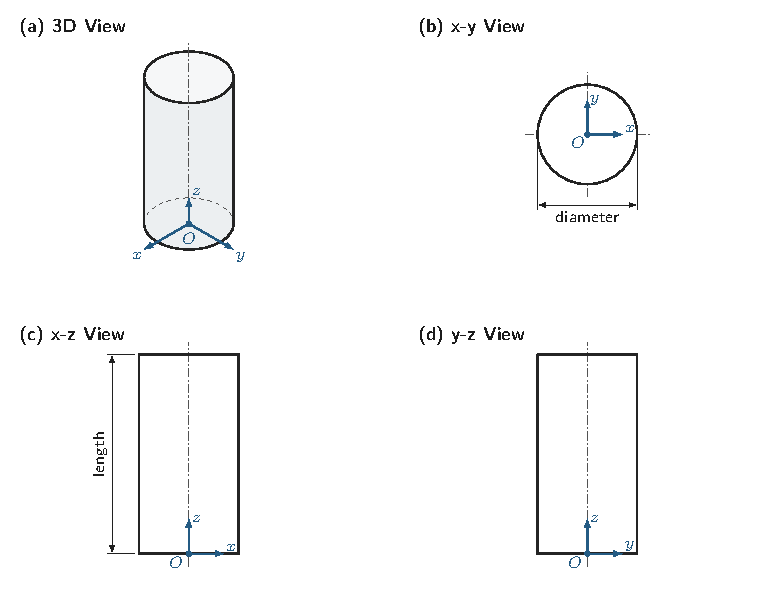
\includegraphics[width=0.7\linewidth]
    {./figs/geometries/cylinder.pdf}
    \caption{Standardized parametrization and local
    coordinate system of the cylinder geometry.}
    \label{fig:cylinder}
\end{figure}

The \texttt{cylinder} geometry represents a right
circular cylindrical specimen. As illustrated in
Fig.~\ref{fig:cylinder}, the local coordinate
system is defined by the right-handed Cartesian
axes $x$, $y$, and $z$.

The origin $O$ is located at the center of the
reference circular end face, corresponding to
$z=0$. The $z$ axis coincides with the longitudinal
axis of the cylinder and extends toward the opposite
end face at $z=\texttt{length}$. The $x$ and $y$
axes define the transverse plane of the circular
cross section.

\paragraph{Independent parameters.}

The geometry is defined by two required parameters,
both expressed in millimeters:

\begin{itemize}
    \item \texttt{length}: longitudinal specimen
    dimension along the local $z$ axis;

    \item \texttt{diameter}: diameter of the
    circular cross section in the local
    $x$--$y$ plane.
\end{itemize}

\paragraph{Geometric constraints.}

Both parameters must be strictly positive.
